\chapter{Introduction}

\section{Particle Physics and the Standard Model}

The main objects of study of Particle Physics are the fundamental constituents of Nature, the particles, and the interactions between them, the forces. 
%1Fundamental particles are those which, to the best of our knowledge, are not actually systems of other particles. 

Starting from the perspective of pre-mid-20th century physics, four fundamental forces between particles, observed from then-known physical phenomena, may be listed: Gravity, between particles with mass; Electrodynamics, between particles with electric charge; the Strong Force, responsible for keeping nucleons together in atomic nuclei; and the Weak Force, responsible for the radioactive decay of nuclei involving the conversion of a proton into a neutron or vice-versa. Around the same time, a suspected set of fundamental particles could comprise the proton, the neutron, the electron and the neutrino. %As we will see, the Standard Model proposes a much larger set of fundamental particles.

The Standard Model of Particle Physics aims to explain natural phenomena starting from a a set of fundamental particles and the mathematical framework, provided by Quantum Field Theories, to describe interactions between them. It was developed over the second half of the 20th century with contributions from many physicists, and is often referred to as the most successful modern physical theory, having produced a variety of theoretical predictions which have been independently
%, and often to great accuracy, 
confirmed through experiment. These include the prediction of several particles before their observation and the famously precise prediction of the anomalous magnetic moment of the electron, which agrees with experiment to roughly one part in $10^{10}$ \cite{Fan_2023}. 
%There is no shortage, however, 
However, there is also no shortage of physical phenomena currently unexplained by the Standard Model, such as gravity, baryon asymmetry (the prevalence of matter over antimatter in the Universe) and dark matter.%, both at the cosmological scale and 

%The \textbf{Standard Model of Particle Physics} provides \textbf{a set of fundamental particles} and the mathematical framework to describe interactions between them, \textbf{Quantum Field Theories}. It was developed over the second half of the 20th century with contributions from many physicists, and is often referred to as the most successful modern physical theory, having produced a variety of theoretical predictions which have been independently confirmed through experiment. However, there is also no shortage of physical phenomena currently unexplained by the Standard Model, such as gravity. 



%mainly at the macroscopic scale with which it was not initially built in mind
%experimentally verified predictions

The set of fundamental particles in the Standard Model differs from the earlier suspected set. In the static quark model, the proton and the neutron were proposed to actually be composite particles, with nucleons being made of three quarks, of up- or down- flavor. Later, particles generated from the interactions between these quarks were added to the composition of the nucleons. A new fundamental particles set candidate arises -- the up-quark, the down-quark, the electron and the neutrino -- which actually make up the first generation of fermions. They are roughly the particles involved in physical phenomena at our energy scale. At greater energy scales, two other generations come into play, each made up of four particles, copies of the first four, differing only in mass. For each fermion, an oppositely-charged copy, its antiparticle, also exists. Additionally, interactions between particles at a distance are always mediated by other particles, with each fundamental force having an associated mediator particle, called a vector boson: the photon for Electrodynamics, the $W$ and $Z$ bosons for the Weak Force, and the gluon for the Strong Force (Fig. \ref{fig:SM_periodic}).

\begin{figure}
    \centering    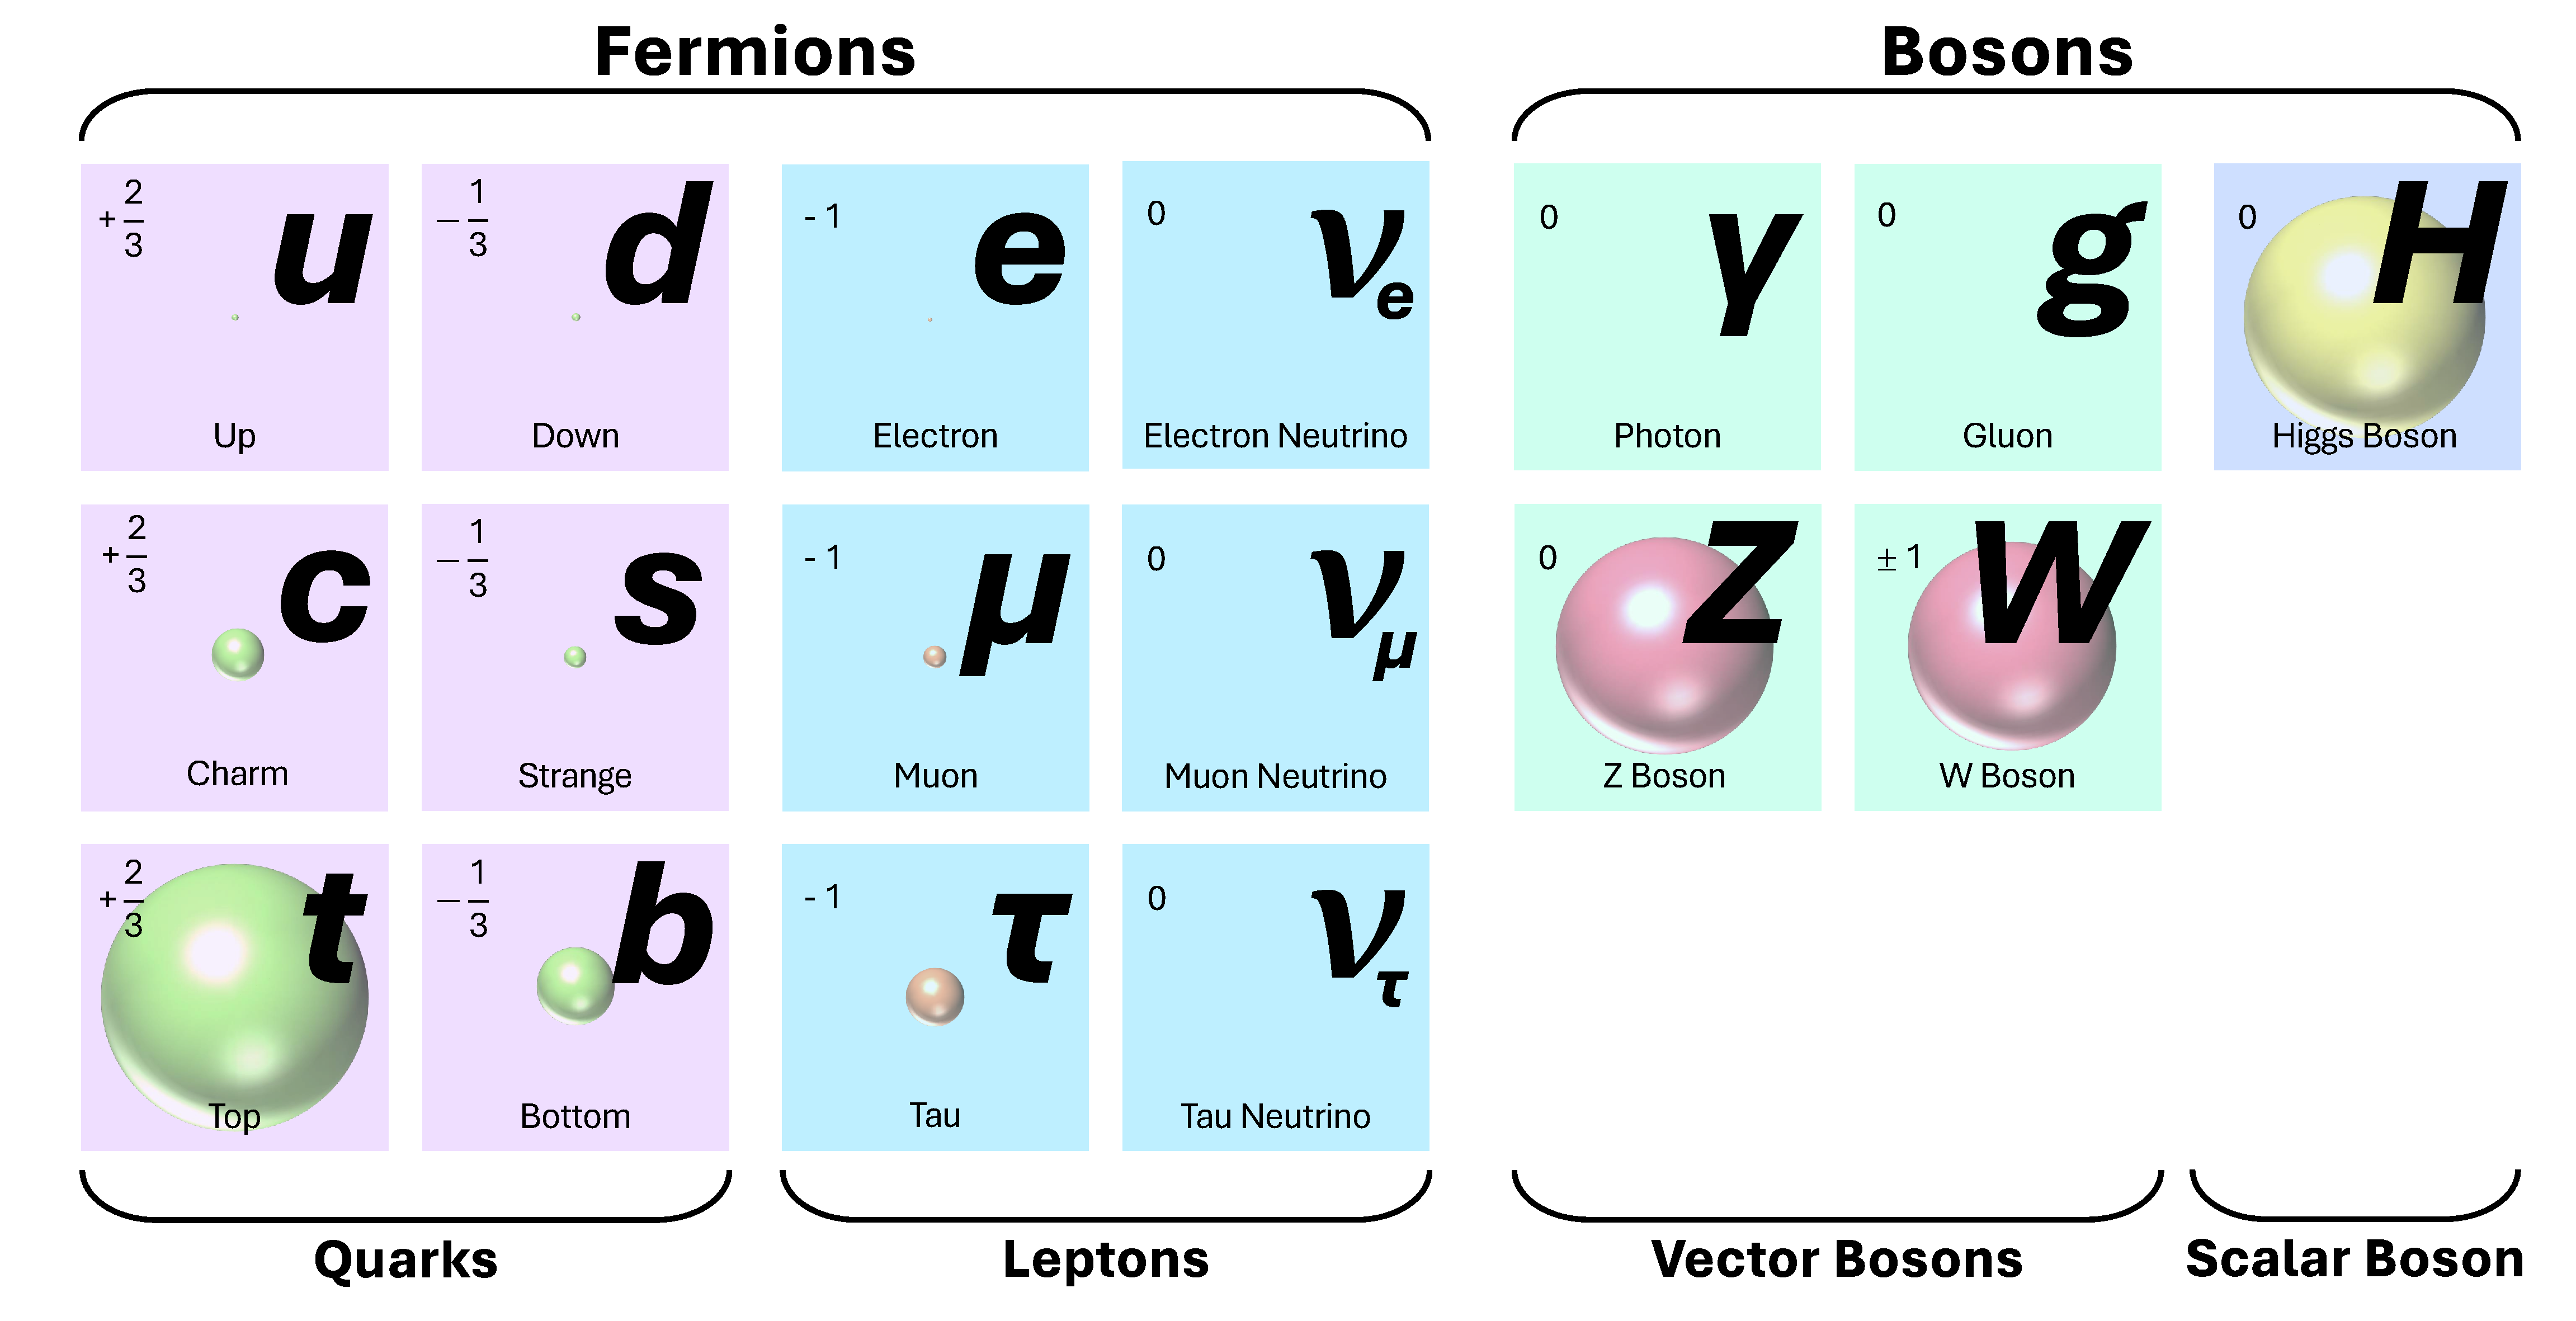
\includegraphics[width=0.9\textwidth]{Figures/version2.pdf}
    \caption{The elementary particles of the Standard Model. For each particle, its charge relative to the electron is shown and its mass is illustrated as proportional to the volume of a coloured sphere.}
    \label{fig:SM_periodic}
\end{figure}

%The fundamental force's relative strengths order them as suggested by their names

%Only the particles with a force's associated charge can experience that force through interaction with its mediator particles. Only electrically charged particles -- the W boson and all fermions, excluding neutrinos -- experience the electromagnetic force by interaction with the photon. All fermions experience the weak force, as they all have weak isospin charge allowing them to interact with the W and Z bosons. Finally, 

The forces' relative strengths allow us to determine which force, out of the ones allowed in a system, is dominant: if the Strong Force has a strength of order $1$, the electromagnetic force's strength is of order $10^{-3}$, the Weak Force's strength is of order $10^{-8}$, and gravity's strength is of order $10^{-37}$. \cite{Thomson:2013} In systems composed of Strong Force-sensitive particles, the Strong Force is taken to dominate, as is the case with nucleons. As stated before, the proton and the neutron are made up of quarks and particles generated by the interactions between them, other quarks and gluons; these components of the nucleons, and of all other hadrons, may be succinctly referred to as partons.

%Something about the Lagrangian??

%\textcolor{blue}{An introduction to the Standard Model of Particle Physics and interaction by particle exchange. Overview of the different kinds of fermions and bosons and the permitted interactions between them.}

	\subsection{The Strong Force}
In systems made up of quarks and gluons, which will be the subject of this work, the Strong Force is the dominant fundamental 
force. %As such, all calculations will set off from the Strong Force's field theory, \gls{QCD}. 

Only particles with color charge experience the Strong Force -- this includes only the quarks and the strong force's own mediator particle, the gluon. This is in contrast with Electrodynamics, where the mediator particle, the photon, does not carry electric charge.
%Colour can be thought of in terms of the more familiar electric charge as a set of three charges: red charge, green charge and blue charge.
%As said before, only particles carrying colour charge feel the strong force. 
Color is actually a set of three charges: red charge, green charge and blue charge. All quarks and gluons have non-zero color charge, and all interactions between them -- and with any other particles -- conserve the total color charge over time. The allowed interactions between quarks and gluons are shown in Fig. \ref{fig:strong_interactions}.

\begin{figure}
  \centering
  \begin{minipage}[c]{0.3\textwidth}    
   \centering
   \begin{tikzpicture}
    \begin{feynman}
    \vertex (c);
    \vertex [above left=of c] (q1) {q};
    \vertex [above right=of c] (q2) {q};
    \vertex [below=of c] (g) {g};

    \diagram* {
    (q1) -- [fermion] (c) -- [fermion] (q2),
    (c) -- [gluon] (g),
    };
    \end{feynman}
\end{tikzpicture}
  \end{minipage}
  \begin{minipage}[c]{0.3\textwidth}
    \centering
    \begin{tikzpicture}
    \begin{feynman}
    \vertex (c);
    \vertex [above left=of c] (g1) {g};
    \vertex [above right=of c] (g2) {g};
    \vertex [below=of c] (g3) {g};

    \diagram* {
    (g1) -- [gluon] (c) -- [gluon] (g2),
    (c) -- [gluon] (g3),
    };
    \end{feynman}
\end{tikzpicture}
  \end{minipage}
  \begin{minipage}[c]{0.3\textwidth}
    \centering 
    \begin{tikzpicture}
    \begin{feynman}
    \vertex (c);
    \vertex [above left=of c] (g1) {g};
    \vertex [above right=of c] (g2) {g};
    \vertex [below left=of c] (g3) {g};
    \vertex [below right=of c] (g4) {g};

    \diagram* {
    (g1) -- [gluon] (c) -- [gluon] (g4),
    (g3) -- [gluon] (c) -- [gluon] (g2),
    };
    \end{feynman}
\end{tikzpicture}
    \end{minipage}
    \caption{The interactions of the Strong Force. Solid, oriented lines represent quarks and "spring" lines represent gluons.}
    \label{fig:strong_interactions}
\end{figure}

%A process where a quark and a gluon exchange momentum and colour charge via exchange of a gluon is illustrated in Fig. \ref{fig:colour_illustrated}. In it, a red-charged quark ($r$) emmits a red-charged and negatively blue-charged gluon ($r\bar{b}$), becoming blue-charged ($b$). The gluon that absorbs it, originally $gb$, becomes $rg$. The total red, green and blue charges are conserved at every point.

%\begin{figure}[h]
%    \centering    \begin{tikzpicture}
    \begin{feynman}
    \vertex (q1) {q};
    \vertex at ($(q1) + (4cm, -0.5cm)$) (a);
    \vertex [right=9cm of q1] (q2) {q};
    \vertex at ($(a) + (+1.5cm, -2cm)$) (b) ;
    \vertex [below=3cm of q1] (g1) {g};
    \vertex [right=9cm of g1] (g2) {g}; 

    \vertex at ($(q1) + (0.2cm, 0.2cm)$) (q11);
    \vertex at ($(a) + (0.2cm, 0.2cm)$) (a1);
    \vertex at ($(b) + (0.2cm, 0.2cm)$) (b1);
    \vertex at ($(g2) + (0.2cm, 0.2cm)$) (g21);

    \vertex at ($(g1) + (-0.2cm, 0.2cm)$) (g12);
    \vertex at ($(b) + (-0.45cm, 0.2cm)$) (b2);
    \vertex at ($(a) + (-0.2cm, -0.2cm)$) (a2);
    \vertex at ($(q2) + (-0.2cm, -0.2cm)$) (q22);

   \vertex at ($(g1) + (0, -0.3cm)$) (g13);
    \vertex at ($(b) + (0, -0.3cm)$) (b3);
    \vertex at ($(g2) + (0, -0.3cm)$) (g23); 


    \diagram* {
    (q1) -- [fermion] (a) -- [fermion] (q2),
    (a) -- [gluon, edge label'=g\(_1\)] (b),
    (g1) -- [gluon] (b)  -- [gluon] (g2),
    (q11) -- [red, charged scalar] (a1) -- [red, charged scalar] (b1) -- [red, charged scalar] (g21),
    (g12) -- [blue, charged scalar] (b2) -- [blue, charged scalar] (a2) -- [blue, charged scalar] (q22),
    (g13) -- [green, charged scalar] (b3) -- [green, charged scalar] (g23), 
    };
    \end{feynman}
\end{tikzpicture}
%    \caption{Feynman diagram representing the scattering of a quark (q) and a gluon (g) via exchange of a gluon (g$_1$), which is emmited by the quark. Time is ordered left to right, and colour charge flow is shown explicitly.}
%    \label{fig:colour_illustrated}
%\end{figure}

The fact that the Strong Force is mediated by a massless boson between particles carrying its associated charge may suggest that it should be quantitatively treated and behave similarly to Electrodynamics. However, this not the case. The crucial difference between the Strong Force and Electrodynamics manifests in the fact that the gluon may interact with itself, while the photon may not. \gls{QCD}, the Strong Force's quantum field theory in the Standard Model, is an SU(3) gauge theory, and the non-abelian nature of the SU(3) group is the origin for the gluon's self-interaction. U(1), the group of the gauge theory for \gls{QED}, is an abelian group, due to which the photon does not interact with itself. This leads to the vastly different observed behaviors of \gls{QCD} and \gls{QED}.
Once a Quantum Field Theory is renormalized, its strength, expressed by its coupling constant -- usually, $e$ for \gls{QED} and $g_S$ for \gls{QCD} --, becomes dependent on the energy scale\footnote{Or, equivalently, its length or time scale.} of the phenomenon being described, $\mu$, earning it the name of ``running coupling''. $e$ acquires a relatively weak dependence on $\mu$, and grows with it. Non-abelian gauge theories, on the other hand, may have their coupling constants decrease with $\mu$; this is the case for $g_S$, which has a strong dependence on $\mu$. Consequently, at low $\mu$, it increases to values that no longer permit handling \gls{QCD} via Perturbation Theory -- the writing of a quantity as a power series in the coupling constant, and the truncation of that power series in order to allow its computation. Since the power of $g_S$ associated with a process grows with the number of Strong Force vertices, this means that in order to calculate any result one would have to sum the contributions of an infinite number of increasingly complex diagrams, as illustrated in Fig. \ref{fig:running_QED_QCD}. 

\begin{figure}
\centering
\begin{align*}
\begin{tikzpicture}[domain=0:2.3, baseline=(a.mid)]
\node [draw=none] at (0,1.1) (a) {};
\draw[->] (-0.2,0) -- (3,0) node[below] {$\mu$};
\draw[->] (0,-0.2) -- (0,2.5) node[left] {$e(\mu)$};
\filldraw[black] (0,1) circle (1pt) node[left] {$\sim \sqrt{\frac{4\pi}{137}}$};
\draw   plot (\x,{1 + \x*\x/45});
\end{tikzpicture}
& \quad \to \quad
\begin{tikzpicture}[baseline=(ctr.base)]
\begin{feynman}[inline=ctr.base)]
\vertex (a1) {e};
\vertex[right=3cm of a1] (a3);
\vertex[below=1.5cm of a1] (b1) {e};
\vertex[right=3cm of b1] (b5);
\vertex at ($(a1)!0.5!(b1)$) (ctr);
\diagram* {
(a1) -- [plain] (a3),
(b1) -- [plain] (b5),
};
\end{feynman}
\end{tikzpicture}
+
\begin{tikzpicture}[scale = 0.7, transform shape, baseline=(ctr.base)]
\begin{feynman}[inline=ctr.base)]
\vertex (a1);
\vertex[right=1.5cm of a1] (a2);
\vertex[right=1.5cm of a2] (a3);
\vertex[below=1.5cm of a1] (b1);
\vertex[right=1.5cm of b1] (b4);
\vertex[right=1.5cm of b4] (b5);
\vertex at ($(a1)!0.5!(b1)$) (ctr);
\diagram* {
{[edges=plain]
(a1) -- (a2) -- (a3),
},
{[edges=plain]
(b1) -- (b4) -- (b5),
},
(a2) -- [photon] (b4),
};
\end{feynman}
\end{tikzpicture}
+
\underbrace{
...+
\begin{tikzpicture}[scale = 0.5, transform shape, baseline=(ctr.base)]
\begin{feynman}[inline=ctr.base)]
\vertex (a1);
\vertex[right=0.5cm of a1] (a2);
\vertex[right=2.5cm of a2] (a3);
\vertex[below=1.5cm of a1] (b1);
\vertex[right=0.5cm of b1] (b2);
\vertex[right=1cm of b2] (b3);
\vertex[right=1cm of b3] (b4);
\vertex[right=0.5cm of b4] (b5);
\vertex at ($(a2)!0.3!(b4)$) (c1);
\vertex at ($(a2)!0.6!(b4)$) (c2);
\vertex at ($(a1)!0.5!(b1)$) (ctr);
\diagram* {
{[edges=plain]
(a1) -- (a2) -- (a3),
},
{[edges=plain]
(b1) -- (b2) -- (b3) -- (b4) -- (b5),
},
(a2) -- [photon] (c1),
(c1) -- [plain, half right] (c2) -- [plain, half right] (c1),
(c2) -- [photon] (b4),
(b2) -- [photon, half left] (b3),
};
\end{feynman}
\end{tikzpicture}
+...
}_\text{may be truncated}	
\\
\begin{tikzpicture}[domain=0.7:2.3, baseline=(a.mid)]
\node [draw=none] at (0,1.1) (a) {};
\draw[->] (-0.2,0) -- (3,0) node[below] {$\mu$};
\draw[->] (0,-0.2) -- (0,2.5) node[left] {$g_S(\mu)$};
\draw[thin, gray,dashed] (1,0) node[below, black] {$\Lambda_{\text{QCD}}$} -- (1,1.5) -- (0,1.5) node[left, black] {$\sim 1$};
\filldraw[black] (1,1.5) circle (1pt);
\draw   plot (\x,{1.5 / \x});
\end{tikzpicture}
& \quad \to \quad
\begin{tikzpicture}[baseline=(ctr.base)]
\begin{feynman}[inline=ctr.base)]
\vertex (a1) {q};
\vertex[right=2.2cm of a1] (a3);
\vertex[below=1.5cm of a1] (b1) {q};
\vertex[right=2.2cm of b1] (b5);
\vertex at ($(a1)!0.5!(b1)$) (ctr);
\diagram* {
(a1) -- [plain] (a3),
(b1) -- [plain] (b5),
};
\end{feynman}
\end{tikzpicture}
+
\begin{tikzpicture}[baseline=(ctr.base)]
\begin{feynman}[inline=ctr.base)]
\vertex (a1);
\vertex[right=1cm of a1] (a2);
\vertex[right=1cm of a2] (a3);
\vertex[below=1.5cm of a1] (b1);
\vertex[right=1cm of b1] (b4);
\vertex[right=1cm of b4] (b5);
\vertex at ($(a2)!0.5!(b4)$) (ctr);
\diagram* {
{[edges=plain]
(a1) -- (a2) -- (a3),
},
{[edges=plain]
(b1) -- (b4) -- (b5),
},
(a2) -- [gluon] (b4),
};
\end{feynman}
\end{tikzpicture}
+...+
\begin{tikzpicture}[baseline=(d1.base)]
\begin{feynman}[inline=d1.base)]
\vertex (a1);
\vertex[right=0.7cm of a1] (a2);
\vertex[right=1.5cm of a2] (a3);
\vertex[right=0.2cm of a3] (a4);
\vertex[below=1.5cm of a1] (b1);
\vertex[right=0.2cm of b1] (b2);
\vertex[right=1cm of b2] (b3);
\vertex[right=1cm of b3] (b4);
\vertex[right=0.2cm of b4] (b5);
\vertex at ($(a3)!0.1!(b4)$) (c1);
\vertex at ($(a3)!0.4!(b4)$) (c2);
\vertex at ($(a3)!0.7!(b4)$) (c3);
\vertex at ($(a2)!0.5!(b3)$) (d1);
\diagram* {
{[edges=plain]
(a1) -- (a2) -- (a3) -- (a4),
},
{[edges=plain]
(b1) -- (b2) -- (b3) -- (b4) -- (b5),
},
(a3) -- [gluon] (c1) -- [gluon] (c2),
(c2) -- [plain, half right] (c3) -- [plain, half right] (c2),
(c3) -- [gluon] (b4),
(a2) -- [gluon] (d1) -- [gluon] (b3),
(b2) -- [gluon] (d1) -- [gluon] (c1),
};
\end{feynman}
\end{tikzpicture}
+...
\end{align*}
\caption{(Left) Rough dependence of the couplings of \glshyperlink{QED} (top) and \glshyperlink{QCD} (bottom) on the energy scale $\mu$ of a studied process. At low $\mu$, $e(\mu)^2/4\pi$ approaches the value of the fine structure constant, $\alpha = e^2/4\pi \approx 1/137$. Below $\Lambda_\text{QCD}\approx \qty{150}{MeV}$, $g_S$ is greater than one, disallowing the truncation of higher-order, more complex terms, the Perturbation Theory technique applicable for a wide range of energy scales in \glshyperlink{QED}. (Right) Examples of the terms in the power series for the interaction between two electrons (top) and two quarks (bottom). For the quark pair, infinitely many diagrams with an increasing number of exchanged particles must be considered.}
\label{fig:running_QED_QCD}
\end{figure}

The case of low energies is equivalent to that of long distances. Color-charged particles separated over long distances are subject to the Strong Force with a large, non-perturbative coupling. As in Fig. \ref{fig:running_QED_QCD}, more complex processes are not necessarily less likely. Thus, gluons exchanged between any two color-charged particles moving away from one other are likely to exchange gluons between themselves and form quark-antiquark pairs ($q\overline{q}$). As such, the total energy stored in the fields between the distancing pair of particles increases until it becomes more energetically favorable for a ($q\overline{q}$) pair to remain between the two original particles, ``screening'' their charges and shortening the interaction distances. After this, if the original particles retain enough momentum to keep moving away from each other, the process repeats until only groups of particles in color singlets (with no overall color charge), such as mesons, protons or neutrons, remain -- hadronization. This is the qualitative explanation for the fact that no isolated color-charged particles, like quarks and gluons, have been observed; this is called color confinement, for which an analytical explanation has yet to be found. Only composite particles, like hadrons, such as the proton and the neutron, have been detected, even though evidence for the existence of quarks and gluons exists.
Conversely, at short distances or high energies, the coupling decreases logarithmically, leading to the	 \gls{QCD} regime called asymptotic freedom, where quarks and gluons can exist isolated and where Perturbation Theory is applicable.
%\textcolor{purple}{Conversely, at high energies Perturbation theory becomes applicable, ASYMPTOTIC FREEDOM}
%, $g_S$ drops off logarithmically for large enough $\mu$;

%One crucial difference between the Strong Force, whose framework is QCD, and Electrodynamics, whose framework is \gls{QED}, is how sensitive each force's strength is to the energy of the process involved. What was previously mentioned as a force's strength is called, in the context of its field theory, its coupling, and is denoted $e$ for \gls{QED} and $g_S$ for \gls{QCD}. When calculating the probability of a certain process, the result will be proportional to powers of each relevant coupling; each power's exponent will be larger the more of that force's interactions occur in the process.% For example, Fig. \ref{fig:colour_illustrated}'s process counts two strong interactions.

%In calculating the probability of a specific set of initial particles turning into a specific set of final particles, one should consider \textit{all} relevant processes. However, if the relevant couplings are appropriately small, it is possible to approximate the result by excluding the more complex processes containing more interactions, as their contribution to the result is proportional to greater powers of the (small) coupling -- Perturbation Theory. \gls{QED}'s coupling remains appropriately small over a wide range of energies, including at low energies. \gls{QCD}'s coupling, however, is more sensitive; it decreases with increasing energy scale and disallows perturbation theory at energies below around $\Lambda_{\text{QCD}}$, a few hundred MeV. Thus, at low energies, one is forced to compute infinitely many processes, impossibilitating a treatment like \gls{QED}'s. The variation of a coupling with the relevant energy scale earns it the name ``running coupling''. 

%A second crucial difference between \gls{QED} and \gls{QCD} is that, while it is possible to observe non-neutral electrically charged particles, like the electron, no free particles with non-zero colour charge are observed. That is, free quarks and gluons are never detected, only colourless composite particles made from them -- hadrons, like the proton. This is called colour confinement, and an analytic explanation for it has yet to be found. 

%A possible qualitative explanation [places the blame on the fact that] the gluon, simultaneously a colour-charged particle and the strong force's mediator, may interact with other gluons (see second and third interactions in Fig. \ref{fig:strong_interactions}). Thus, it is attracted to 
%The photon, not being electrically charged, cannot interact with other photons.


%A crucial difference lies in the fact that a gluon, simultaneously a colour-charged particle and the strong force's mediator, may interact with other gluons (see second and third interactions in Fig. \ref{fig:strong_interactions}). The photon, not being electrically charged, cannot interact with other photons.

%\textcolor{blue}{A closer exposition on quarks and gluons, and QCD and the unique properties of the strong force (confinement, running coupling, range).}

\subsection{Jets}

In Particle Physics experiments at colliders, a high energy quark or gluon is often produced which travels away from its birthing interaction vertex towards the surrounding particle detectors. Eventually, however, the distance between it and other color-charged particles grows until the process of hadronization takes over and a shower of colorless hadrons is generated. This shower of hadron lies in a ``cone'' around the original quark or gluon's momentum direction and is called a jet. It is the hadrons in this jet which actually reach the detectors, and several of its quantitative characteristics provide information on its founding particle. For example, the  sum of the hadrons' four-momenta returns the founding particle's four-momentum. The process of jet formation from two receding quarks is illustrated in Fig. \ref{fig:hadronisation}. 

%If a quark or a gluon (a parton)
%is energetic enough, it may propagate while not being part of a colourless hadron. The energies associated with the colour fields generated between it and other colour-charged particles grow quickly with their separation until the creation of a quark-antiquark pair (q$\bar{\text{q}}$) between them -- which "screens" their different charges -- becomes more energetically favourable. As this set of partons continue to separate, more pairs are created until the particles reach a low enough energy  to be forced to confine into colourless hadrons (Fig. \ref{fig:hadronisation}). During this process, quarks may also radiate gluons or gluons may turn into q$\bar{\text{q}}$ pairs as well. 
%Thus, a highly energetic parton originates a set of hadrons which lie in a "cone" around the original parton's momentum direction -- a jet. It is these hadrons which are detectable, and the sum of their 4-momenta equals the original parton's 4-momentum.
%Thus, a highly energetic parton originates a set of hadrons whose momenta lie in a "cone" around the original parton's momentum; the sum of their 4-momentum equals the original particle's 4-momentum.


\begin{figure}
    \centering
    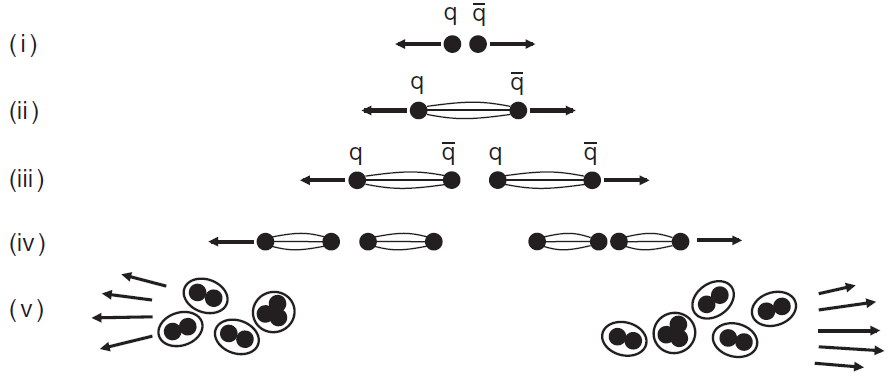
\includegraphics[width=0.7\textwidth]
    {Figures/hadronisation.PNG}
    \caption{The generation of two jets from a separating q$\bar{\text{q}}$ pair. From \cite{Thomson:2013}.}
    \label{fig:hadronisation}
\end{figure}

%The process through which the observed hadrons are formed out of "lone" quarks and gluons is called hadronisation. When


%\textcolor{blue}{An introduction to Jets following from the context above.}

\section{Heavy Ion Collisions}

At collider experiments, beams of particles are accelerated and made to collide with each other, 
%so the wreckage
and the products of the collisions are analysed in order to gain insight into the interactions that took place.

When it comes to the study of the Strong Force, the interest is in gathering data relating to the interactions of quarks and gluons. In choosing what species of particles to accelerate and collide, it may be desirable for strong force-sensitive particles to only be products of the collision, or to be present from the beginning, forming the colliding beams. In the second case, only color-neutral composite particles are available due to color confinement, and the most readily available ones are the nuclei of atoms, the simplest of which is the proton, $p$; heavier ones, like gold and lead, are dubbed heavy ions, and are denoted by $A$. The focus of this work will be on \glspl{HIC}, also know as $AA$ Collisions, as they produce the appropriate conditions for the formation of the \gls{QGP}, which will be discussed further ahead.

\glspl{HIC} are performed at CERN's \gls{LHC} in Geneva and at  Brookhaven National Laboratory's \gls{RHIC} in Upton, New York.  At these colliders, beams of hadrons are accelerated in opposite directions to close to the speed of light. At the highest energies attainable at the \gls{LHC}, the Lorentz factor corresponding to the hadrons' velocities is of around $\gamma \approx 2500$; as such, they experience length contraction of the same factor and become very thin disks, as opposed to approximate spheres. The \gls{CM} frame energy of these collisions is denoted by $\sqrt{s}$. \cite{Busza_big_picture_2018} Fig. \ref{fig:HI_CM_coll} represents a heavy ion collision in the CM frame.

\begin{figure}
	\centering
	\begin{tikzpicture}
	\filldraw[color=gray!20] (0,1) rectangle (3,-1);

	\filldraw[fill=red!20] (0,0.5) ellipse (0.3 and 1.5);
	\filldraw[fill=red!20] (3,-0.5) ellipse (0.3 and 1.5);
	\node at (0,0.5) [gray] {$\times$};
	\node at (3,-0.5) [gray] {$\times$};
	\draw[-{Latex[length=3mm]},thick] (0,0.5) -- (1.5,0.5) node[midway,above] {$\vec{p}$};
	\draw[-{Latex[length=3mm]},thick] (3,-0.5) -- (1.5,-0.5) node[midway,below] {$-\vec{p}$};
	\draw [|-|,color=gray] (-0.5,0.5) -- (-0.5,2) node[midway,left] {$R$};
	
	\filldraw[color=red!20] (6,0.5) circle (1.5);
	\filldraw[color=red!20] (6,-0.5) circle (1.5);
	\draw (6,0.5) circle (1.5);
	\draw (6,-0.5) circle (1.5);
	\node at (6,0.5) [gray] {$\times$};
	\node at (6,-0.5) [gray] {$\times$};
\end{tikzpicture}
	\caption{Non-central \glshyperlink{HIC} in the \glshyperlink{CM} frame -- side (left) and transverse (right) views. Ions are represented as spheres which are length-contracted (not to scale) in the direction of their 3-momentum. Typical heavy ion radii (gold, lead) are of the order $R \approx \qty{7}{fm}$. For non-central collisions, the overlap region is lenticular.}
	\label{fig:HI_CM_coll}
\end{figure}


%\begin{figure}[h]
%    \centering
    %\includegraphics[width=0.3\textwidth]{example-image-a}
%    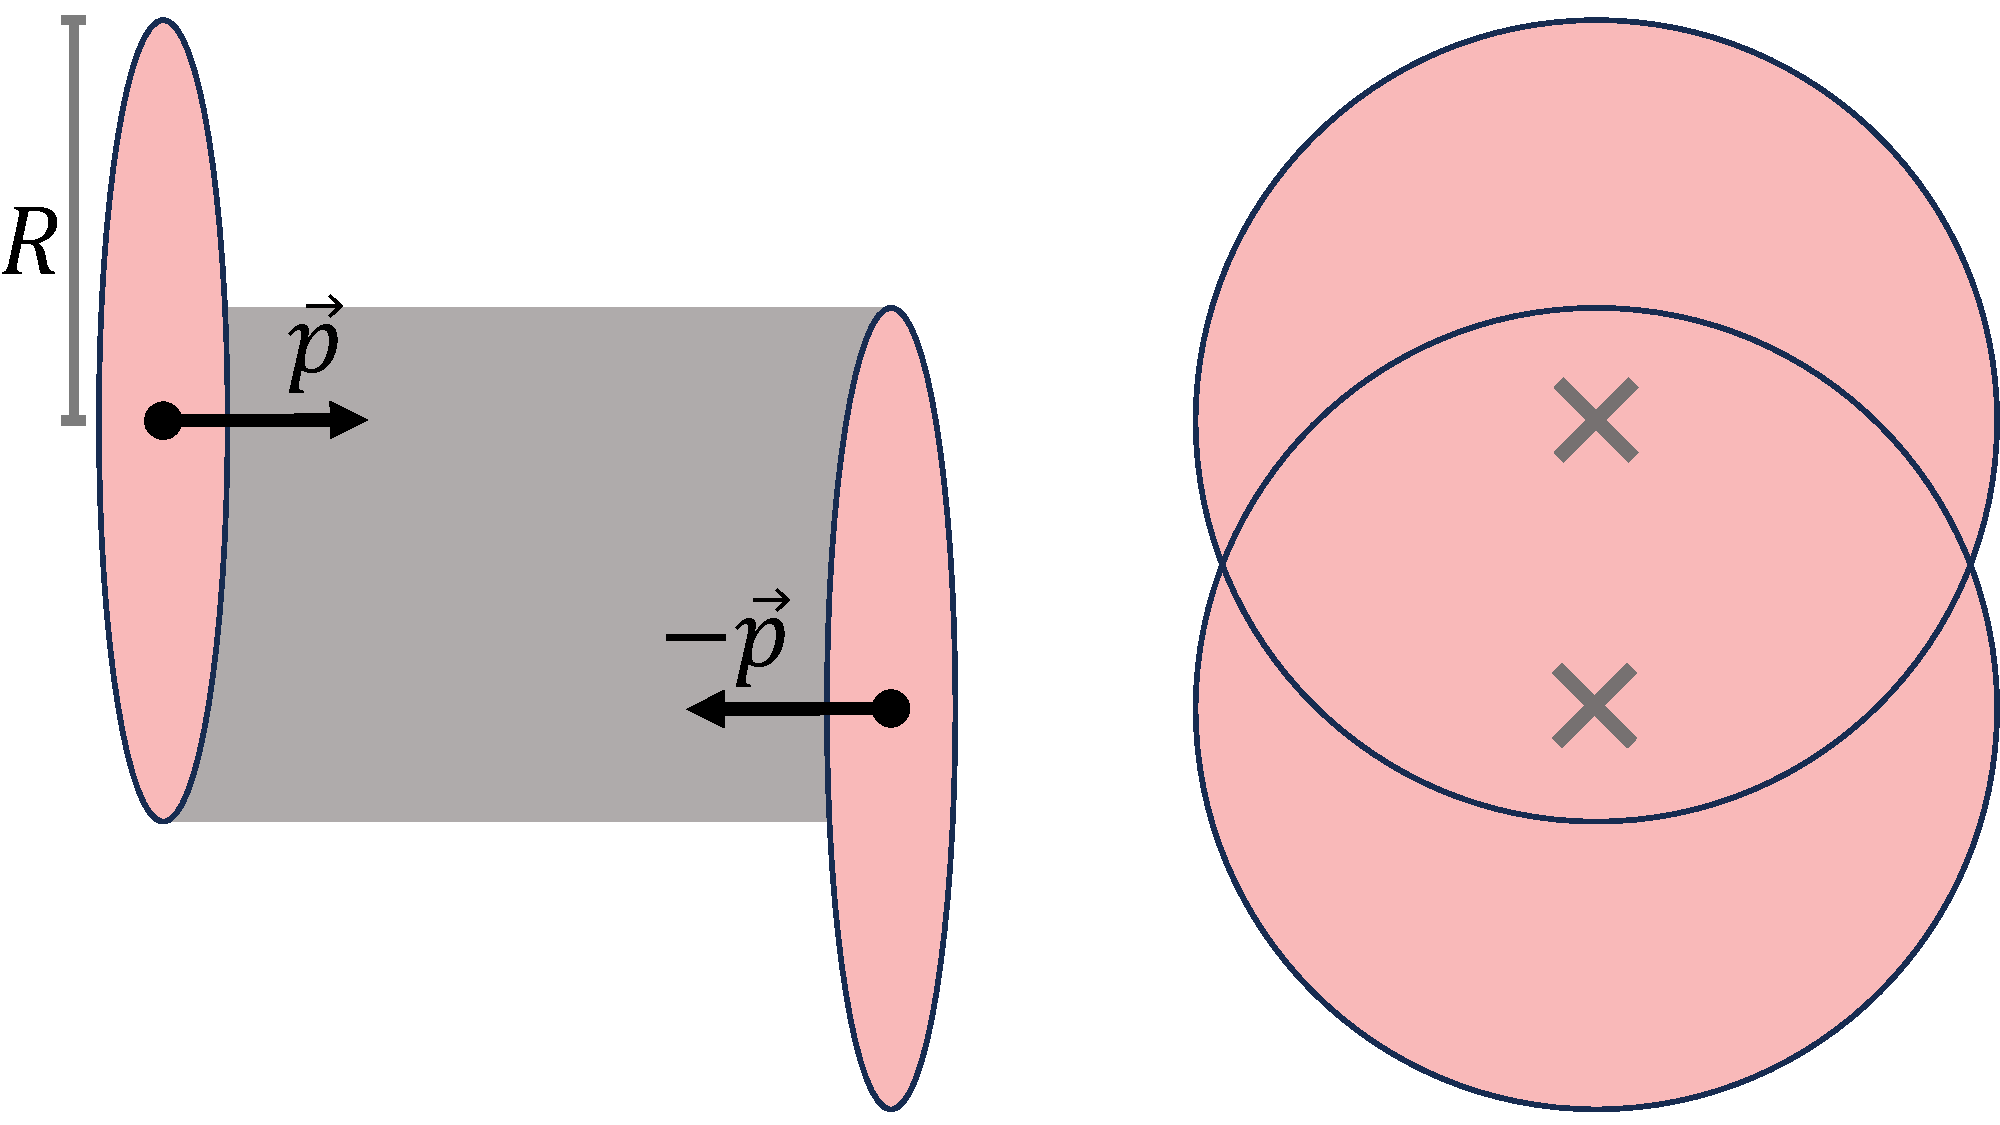
\includegraphics[width=0.5\textwidth]{Figures/HI_CM_coll.pdf}
%    \caption{Non-central heavy ion collision in the CM frame -- side (left) and transverse (right) views. Ions are represented as spheres which are length-contracted (not to scale) in the direction of their 3-momentum. Typical heavy ion radii (gold, lead) are of the order $R \approx 7$ fm. For non-central collisions, the overlap region is lenticular.}
%    \label{fig:HI_CM_coll}
%\end{figure}

The beams are made to collide at points of the accelerator equipped with detectors, which are mounted cylindrically around the accelerator tube. Consequently, only particles produced in the collision with enough transverse momentum reach the detectors, while other particles continue along the accelerator. As said before, no free quarks or gluons are detected, and any high energy partons which may have been produced hadronise and form jets before reaching the detectors.

%OBSERVABLES: jets from particles which acquired high transverse momentum.\cite{Busza_big_picture_2018}

\medskip
As for the region of the collision, the high density of energies generated allows reaching exotic states of quark-gluon matter very distinct from the familiar ones. Fig. \ref{fig:QCD_phase_diagram} presents a possible phase diagram for \gls{QCD} matter. Its state variables are temperature, $T$, which is related to energy density in volume, and baryon number chemical potential, $\mu_B$, which translates into the excess in number of quarks over antiquarks. 

Familiar nuclear matter is present in the diagram within the hadron gas phase at low temperatures and higher $\mu_B$, as protons and neutrons contain a surplus of quarks over antiquarks. Near the vertical axis ($\mu_B\approx 0$, a good approximation for some of the matter produced in \glspl{HIC} at \gls{RHIC} and the \gls{LHC}), increasing the temperature of the hadron gas leads to a smooth transition into the \gls{QGP}, a strongly-coupled fluid-like state of matter made of unconfined quarks and gluons, and the subject of the next section. Continuing upwards along the axis, although not represented in the phase diagram, another smooth transition into a gas-like, rather than fluid-like, \gls{QGP} is predicted. Away from the vertical axis, it is posited that, upwards of some critical value of $\mu_B$, the mentioned transition from a hadron gas into the \gls{QGP} becomes a first order phase transition rather than a smooth one. Searches for this critical point can be made by studying the cooling of droplets of \gls{QGP} formed in \glspl{HIC} at lower and lower energies (see different paths drawn by matter for different $\sqrt{s}$ values). It is further posited that, for great enough $\mu_B$, a color superconductor phase is reached. \cite{Busza_big_picture_2018}

\begin{figure}
    \centering
    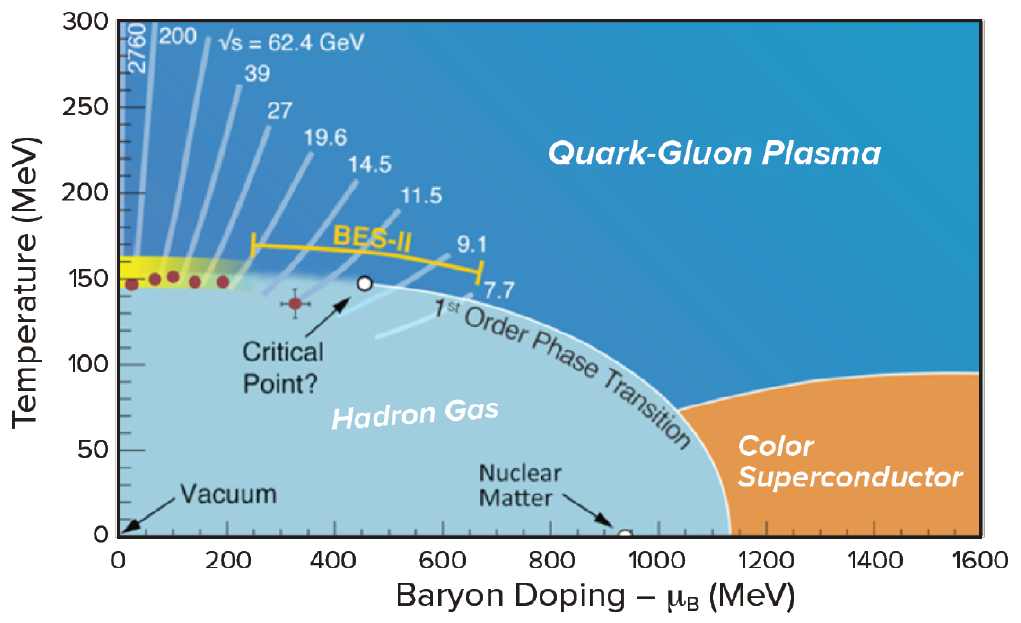
\includegraphics[width=0.5\textwidth]{Figures/QCD_phase_diagram.PNG}
    \caption{A possible \glshyperlink{QCD} phase diagram. Also shown are lines representing the path drawn by cooling \glshyperlink{QGP} droplets from \glshyperlink{HIC} at different $\sqrt{s}$ and expected paths from the then-upcoming phase II of \glshyperlink{RHIC}'s Beam Energy Scan. From \cite{Busza_big_picture_2018}.}
    \label{fig:QCD_phase_diagram}
\end{figure}

%\textcolor{blue}{Description of a heavy ion collision in a particle accelerator - basic kinematics, relativistic contraction. Brief description of what is measurable and observable from a collision. Discussion of the QCD phase diagram.}

\subsection{The Quark-Gluon Plasma}
\label{sec:QGP}

Studying the properties of the \gls{QGP} is of great interest. It was the Universe's first form of complex matter, and can also be thought of as the simplest form of complex matter, since it is a fluid whose constituents interact directly according to the rules of QCD (in the perturbative regime); these are fundamental, rather than effective, interactions, so the study of the \gls{QGP} is of great importance for the understanding of \gls{QCD}.

The \gls{QGP} is formed in \glspl{HIC} as the two nuclei move away from each other post-encounter. During the collision, the constituent partons (quarks and gluons) of both nuclei interact in the overlap region via mostly soft (low) momentum exchanges\footnote{Some hard (high momentum exchange) interactions do occur, which allow for some partons to acquire high transverse momentum. These will serve as important probes of the QGP as will be seen further ahead.} and some color exchanges. As they move away post-collision,
partons from different nuclei exchange gluons, since there was exchange of color between the nuclei. These gluons decay into other gluons and q$\bar{\text{q}}$ pairs in the middle region. The medium created between the separating nuclei is
 %known to 
 energetic enough not to hadronize but not enough for the constituent partons to be free from each other; they are instead strongly coupled, forming a "soup" that is well described as a relativistic hydrodynamic fluid by the time the nuclei are about \qty{2}{fm} apart, at time \qty{1}{fm/c} post-collision. It is characterised by a viscosity to entropy density ratio $\eta / s \approx 1/4\pi$, in units with $\hbar=k_B=1$, which is the smallest of any known fluid.
 New \gls{QGP} continuously forms at later and later times in the wake of the receding nuclei, because it originates from increasingly fast partons which suffer greater time dilation. Once formed, each volume element of \gls{QGP} expands and cools, driven by the initial pressure, until it reaches a low enough energy density which forces it to hadronize. Part of the ensuing cloud of hadrons then ends up with a momentum oriented towards the surrounding detectors. \cite{Busza_big_picture_2018} Fig. \ref{fig:coll_frames} shows snapshots from an animation representing a central \gls{HIC}.

\begin{figure}
    \centering
    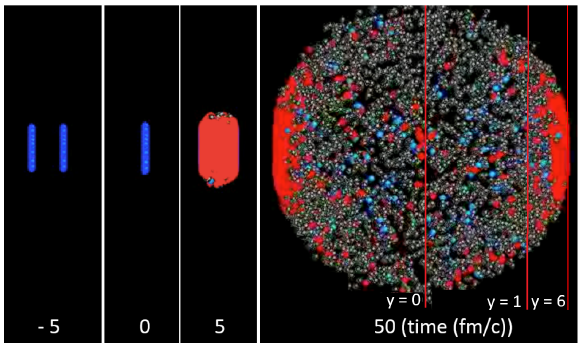
\includegraphics[width=0.5\textwidth]{Figures/coll_frames.PNG}
    \caption{Snapshots from an animation representing a $\sqrt{s}=\qty{2.76}{TeV}$ lead-lead central collision. Hadrons are represented by blue and grey spheres and QGP is shown in red. In the final frame, at time 50 fm/c, lines over particles with the same rapidity, $y$, a function of their distance to the transverse plane containing the center of the collision, are shown. From \cite{Busza_big_picture_2018}.}
    \label{fig:coll_frames}
\end{figure}

The \gls{QGP} formed at these collisions is too small and short-lived to be observed directly, so its mentioned properties have been deduced indirectly from the available observables. These include: 1) The number of produced charged particles and its dependence on $\sqrt{s}$ and the species of nuclei used. 2) The azimuthal distribution of energy deposited in the detectors being anisotropic, which suggests a fluid-like, low viscosity, nature for the \gls{QGP}\footnote{If the QGP were gas-like, azimuthal anisotropies arising from the non-uniform distribution of partons in the nuclei and the lenticular shape of the overlap region would fade away as it expands.}. 3) The production rates of (charm containing) $J/\psi$ and (bottom containing) $\Upsilon$ mesons, which suggest they traverse a medium where partons are unconfined. 4) Lastly, the metrics of hard probes -- partons with high transverse momentum, $p_T$, originating from rare hard scatterings at the beginning of the collision -- which traverse the QGP, losing energy to it in a phenomenon known as jet quenching and creating a wake. \cite{Busza_big_picture_2018}

For the present work, the focus will be on this last avenue for gaining knowledge on the \gls{QGP}. The existence of the \gls{QGP} may be inferred from data on the jets founded by the mentioned high-$p_T$ partons. If there were no \gls{QGP}, a \gls{HIC} could be thought of as equivalent to a certain number $pp$ collisions\footnote{Collisions between two protons.}, $N_\text{coll}$, determined by the centrality of the \gls{HIC}. This approach works well when comparing the number of \mbox{high-$p_T$} photons and $Z$ bosons, which are \textit{not} Strong Force-sensitive, produced in \glspl{HIC} \textit{vs.} $pp$ collisions. However, performing the same comparison regarding high-$p_T$ jets returns that the number and energy of high-$p_T$ jets is lower than expected, suggesting quenching by a medium. Furthermore, the amount of energy lost (around \qty{10}{GeV}), given the small length scales of the medium, suggests an enormous stopping power, which points to the strongly-coupled nature of the \gls{QGP}. 



\subsection{The Pre-Hydrodynamic Phase}

The above discussion has left out concerns about the behavior of the medium \textit{before} it becomes hydrodynamic and reaches equilibrium. If one is hoping to extract information about the \gls{QGP} from probes which traversed it but may have been formed prior to its hydrodinamization, then it is important to assess how they may be affected by the preceding medium, and by how this preceding medium evolves into the initial conditions of the \gls{QGP}.

This will be the concern of the present work. \textcolor{purple}{[Summary of what will be done.]}

%As mentioned in section \ref{sec:QGP}, partons with high transverse momentum, $p_T$, originating from rare high-momentum transfer scatterings at the very beginning of an $AA$ collision may be used as probes into the QGP, viewing as they and the jet they produce must traverse it before reaching the detectors. As they do, they lose energy to it, suffer small deflections, and are posited to create a wake in the QGP. The amount of energy lost(about 10 GeV), given the small length scales of the medium, suggest an enormous stopping power, which is use to argue for the strongly coupled nature of the QGP. \cite{Busza_big_picture_2018} 

%Furthermore, it is found that the number of high-$p_T$ photons and $Z$ bosons from an $AA$ collision is consistent with thinking of an $AA$ collision as a set of $N_{\text{coll}}$ $pp$ collisions, where $N_{\text{coll}}$ is the expected number of nucleon collisions within the hard ion collision. This is no longer the case for the number of high-$p_T$ jets produced, which is much less than what would be predicted from the same reasoning, once again evidencing the strong stopping power of the QGP. \cite{Busza_big_picture_2018}

%\subsection{Glasma and The Colour Glass Condensate}

\textcolor{purple}{$\times$}

%\textcolor{gray}{It is useful to start by thinking about what the conditions are like in the incoming nuclei themselves. They are collections of protons and neutrons (nucleons), which in turn are populated by partons: three valence quarks (uud for the proton and udd for the neutron) and a "sea" consisting of gluons (which are constantly being exchanged between partons) and q$\bar{\text{q}}$ pairs created out of gluons. Within a nucleon, the probability distribution for finding a given parton with a fraction $x$ of the nucleon's total momentum is given by its Parton Distribution Function (PDF). Knowledge of the internal structure of nucleons, and therefore PDFs, has been built via Deep Inelastic Scattering (DIS) experiments, where a projectile (for example, an electron) is made to scatter off a nucleon, probing it. Altering the energy of the projectile changes its resolution of the internal structure of the nucleon. In a qualitative picture, a more energetic probe is subject to greater time dilation and is able to interact with shorter-lived components of the nucleon, which carry a smaller fraction of its momentum (smaller $x$). \cite{gelis2011initial} As such, PDFs acquire greater values for small $x$ when the probe energy is increased. \cite{Busza_big_picture_2018} \cite{gelis2011initial}} %say how this is especially true for gluons

%The linear Balitsky-Fadin-Kuraev-Lipatov (BKFL) equation governs how the (non-integrated over transverse momentum) gluon density evolves with $x$ at a fixed energy scale. According to this equation, the gluon density explodes near $x=0$, but it is unreasonable for this growth to continue indefinitely. As such, the equation is changed by adding a non-linear term translating gluon recombination, to slow down the growth. This is known as gluon saturation and occurs when gluon density is of the order of $1/\alpha_S = 1/{g_S}^2$. \cite{gelis2011initial}

%In the context of $AA$ collisions, the ions travel at ultrarelativistic speeds, so their PDFs are dominated by low-$x$ gluons, which exist at the saturated gluon density. \cite{Busza_big_picture_2018} Under these conditions, the Colour Glass Condensate (CGC) emerges as an adequate effective theory for describing QCD in the saturation regime. The CGC can be considered a semi-classical approach, where the partons in the nucleons are separated into low- and high-$x$ categories. The low-$x$, saturated gluons are treated as classical colour fields ruled by the classical Young-Mills equations and the high-$x$ partons are treated as static colour field sources \cite{Marquet_2014}. This because, from the point of view of the time scales of the short-lived low-$x$ gluons, high-$x$ partons are nearly static. 

%The positions of these sources within the nucleons and their evolution with time are unknown. This problem is overcome by assuming that the distributions of colour charge (the sources) in different nucleons are uncorrelated, which is supported by colour confinement. Then, to get a snapshot of the distribution of the colour charge in the Lorentz-contracted ion, the uncorrelated distributions of a number of longitudinally-alligned nucleons needs to be summed over; this allows for the application of the Central Limit Theorem, providing a form for the distribution of the static colour charge in large nuclei. \cite{gelis2011initial} This specific method for obtaining the static charge distribution is part of the McLerran-Venugopalan Model.



%\textcolor{blue}{Brief presentation of Glasma; the differences between QGP and Glasma (time where they exist after a collision, hydrodynamisation). Why are we interested in knowing more about Glasma.}
